%%%%%%%%%%%%%%%%%%%%%%%%%%%%%%%%%%%%%%%%%
% Journal Article
% LaTeX Template
% Version 1.3 (9/9/13)
%
% This template has been downloaded from:
% http://www.LaTeXTemplates.com
%
% Original author:
% Frits Wenneker (http://www.howtotex.com)
%
% License:
% CC BY-NC-SA 3.0 (http://creativecommons.org/licenses/by-nc-sa/3.0/)
%
%%%%%%%%%%%%%%%%%%%%%%%%%%%%%%%%%%%%%%%%%

%----------------------------------------------------------------------------------------
%	PACKAGES AND OTHER DOCUMENT CONFIGURATIONS
%----------------------------------------------------------------------------------------

\documentclass[twoside]{article}

\usepackage{lipsum} % Package to generate dummy text throughout this template

\usepackage{graphicx} 
\usepackage[]{algorithm2e}


\usepackage[sc]{mathpazo} % Use the Palatino font
\usepackage[T1]{fontenc} % Use 8-bit encoding that has 256 glyphs
\linespread{1.05} % Line spacing - Palatino needs more space between lines
\usepackage{microtype} % Slightly tweak font spacing for aesthetics

\usepackage[hmarginratio=1:1,top=32mm,columnsep=20pt]{geometry} % Document margins
\usepackage{multicol} % Used for the two-column layout of the document
\usepackage[hang, small,labelfont=bf,up,textfont=it,up]{caption} % Custom captions under/above floats in tables or figures
\usepackage{booktabs} % Horizontal rules in tables
\usepackage{float} % Required for tables and figures in the multi-column environment - they need to be placed in specific locations with the [H] (e.g. \begin{table}[H])
\usepackage{hyperref} % For hyperlinks in the PDF

\usepackage{lettrine} % The lettrine is the first enlarged letter at the beginning of the text
\usepackage{paralist} % Used for the compactitem environment which makes bullet points with less space between them

\usepackage{abstract} % Allows abstract customization
\renewcommand{\abstractnamefont}{\normalfont\bfseries} % Set the "Abstract" text to bold
\renewcommand{\abstracttextfont}{\normalfont\small\itshape} % Set the abstract itself to small italic text

\usepackage{titlesec} % Allows customization of titles
\renewcommand\thesection{\Roman{section}} % Roman numerals for the sections
\renewcommand\thesubsection{\Roman{subsection}} % Roman numerals for subsections
\titleformat{\section}[block]{\large\scshape\centering}{\thesection.}{1em}{} % Change the look of the section titles
\titleformat{\subsection}[block]{\large}{\thesubsection.}{1em}{} % Change the look of the section titles

\usepackage{fancyhdr} % Headers and footers
\pagestyle{fancy} % All pages have headers and footers
\fancyhead{} % Blank out the default header
\fancyfoot{} % Blank out the default footer
\fancyhead[C]{CS144 Spring 2014: Final Project, SmarteRun} % Custom header text
\fancyfoot[RO,LE]{\thepage} % Custom footer text

%----------------------------------------------------------------------------------------
%	TITLE SECTION
%----------------------------------------------------------------------------------------

\title{\vspace{-15mm}\fontsize{24pt}{10pt}\selectfont\textbf{SmarteRun: Coding The Portable Coach}} % Article title

\author{
\large
\textsc{Mark Grozen-Smith, Neel Patel, Buffalo Hird}\\[2mm] % Your name
\normalsize Harvard University \\ % Your institution
\vspace{-5mm}
}
\date{5/12/14}

%----------------------------------------------------------------------------------------

\begin{document}

\maketitle % Insert title

\thispagestyle{fancy} % All pages have headers and footers

%----------------------------------------------------------------------------------------
%	ABSTRACT
%----------------------------------------------------------------------------------------

\begin{abstract}

\noindent The pairing of physical activity and music is a natural, common occurrence in modern society.  Today, there are many smartphone and smart device applications focused on this pairing, specifically catering towards runners. Currently, these applications make no attempt to combine music and running in a novel way, instead allowing only for both activities to occur simultaneously. As the prevalence of smart devices continues to alter the technological landscape, the opportunity for the union of this pair is becoming more feasible.  We consider psychological studies that consider the rhythmic nature of human exercise and the effects of music upon this rhythm  We then synthesize a model by which previous activity can predict future run performance and capabilities. We then analyze these predictions and discuss further improvements which can be made to our models. We conclude with the application of this predictive model to music playback and the ability to cater music at speeds which accentuate runners' performance and create the running coach athletes didn't know they had.

\end{abstract}

%----------------------------------------------------------------------------------------
%	ARTICLE CONTENTS
%----------------------------------------------------------------------------------------

\begin{multicols}{2} % Two-column layout throughout the main article text

\section{Introduction}

\lettrine[nindent=0em,lines=3]{B} eyond food, drink, and sleep, the next most essential facet of life is physical exercise. The most common form of exercise is running, but many find it hard to truly stick to a running regime or properly challenge themselves. People who lift weights often stick to rules with concrete results such as increasing their maximum lift every 2 weeks by 5\%, but running is much more difficult to systematize with quantifiable deliverables as it isn't broken up into repetitions or sets. Other than sprinters, a run is a run. A person leaves the start of the run, then at some point later, they end their run. Without someone watching the runner and giving feedback as to how they are doing, little progress is likely to come out of this exercise. \\

This is a problem many are interested in solving. With the insurgence of mobile apps, a number of them have reached success in providing real-time and even overall summarizing data during and at the end of a run. RunKeeper and MapMyRun are the two top apps, but they don't provide much more than a map of where the user has run with an instantaneous and average speed. There are no apps out there which give normative data on how a runner should be running to reach goals. In this day and age with machine learning capabilities surpassing many humans, there should be an app which watches how the user runs and, using data from past runs and the current run's parameters, recommends how a runner should proceed from that moment. Additionally, it would be good if the app provide motivation or somehow otherwise encouraged the runner to maintain the recommended pace. \\

	SmarteRun is a project attempting to address these needs. By using GPS data of a person's run, the app keeps track of each run's speed vs. time relation as well as the total length of the run. Then, during the run, the app uses machine learning to combine data from past recorded runs and determine a reasonable speed the runner should hold for the rest of the run. This project is about the investigation into how to properly combine past data and effectively deliver a proper recommendation speed. The intent is that this speed would be translated into a pace and ultimately used to decide a song that should be played to subliminally push the runner, thereby giving them the coach they don't even realize they have. 


%------------------------------------------------

\section{Background}
\indent The original idea for this project came from an observation that most runners listen to music. The reason most do is probably because music is entertaining and something to think about while running. It turns out that this distraction is more than just entertainment for an unfocused runner. In an article from the Journal of Sport Behavior, they discuss that music can actually allow for improved performance. There are a few basic reasons for this enhanced performance. \\

	First, psychological theories posit that the human mind only has so much attention it can utilize at once. It follows, then, that the more one splits their attention, the less they can pay attention to any one thing. In runners, this leads to a limited amount of attention they can devote to "feeling the pain" of a run if they are listening to music. Without the music, they may just focus on how hard they are working, but with music, the music drowns out the difficulty of the exercise. This idea is backed up in research as studies found a causal link between playing music and feeling a lower rate of perceived exertion. \\
	
	Similar to the diverted attention theory, the psychological effect of dissociation plays a role as well. Rather than just cutting attention from the work out due to a limited potential of focus, music also allows people to escape the workout and dissociate themselves from the struggle. This effect enables runners to meditatively and mechanically go through their run without really noticing, and thus the effects on their body are mitigated. Almost surprisingly, the physiological strain is even assuaged. Studies found a causal link between music and lower heart rates during medium intensity exercise, which allowed for higher intensity, or higher endurance workouts. This may be due to an inhibition of fatigue feedback, or just essentially the placebo effect of the person just not realizing they are working as hard. Either way, music undoubtedly has valuable physical and psychological effects. \\
	
	Finally, the journal article cited research into mood and rhythm effects of music. The mood of over a hundred russian weight lifters was polled and every single one of them said music made them enjoy their work out more. Over 95\% said that music helped them look forward to workouts as well as increase the volume and intensity of those workouts. Again, music has profound effects on the psyche of an athlete. On the topic of rhythm, it has been found that humans naturally assume the rhythm provided by an external source. In the context of SmarteRun, this means that any reasonable, recommended pace can be imposed on the runner by playing music with the right beat. \\
	
	All in all, it is clear that music is effective in influencing the performance of runners, providing value to benchmark performance, enjoyment of the workout, and regularity of keeping to a regimen. (Karageorghis)\\
	
	Other attempts at using past exercise data to predict future performance are scarce, however there is one major example. In 2013, the Boston Marathon had to be shutdown before many participants could finish due to an act of terrorism. In order to determine run times for the unfinished runners, a group from the Harvard School of Public Health was employed to predict performance for the incomplete times. The investigation determined the best approach was to use a K-nearest-neighbor algorithm searching for similar other runs in a dataset of past run data, and then combining them to extrapolate to the rest of the run. This method far exceeded the "constant pace" assumption others had proposed, as well as several other statistical attempts such as the ANOVA method. This method worked very well as it predicted 98\% of runs to within 10 minutes. While this is a large error for normal runs, 10 minutes is small on marathon scale. For 80\% of runners, that error is cut in half. (Hammerling)\\
	
	Given this research, we have validated the idea of using past data to predict future run performance as well as using music to improve and influence the runner's experience. \\

%------------------------------------------------

\section{Implementation}

\indent We implemented our algorithms in Python 2.7, utilizing a mix of object-oriented design and iterative helper functions. We attempt to accomplish two main tasks 1) Given a set of previous runs, provide a good prediction for how a runner should perform in a subsequent run of a certain distance 2) Given a certain distance elapsed in a run, give a reasonable prediction for how a runner should perform based on previous data and whether they intend to match, exceed, or relax compared to this data. We represent our runs using a plot R(x,y,z) in 3-dimensional space where our dimensions are defined as follows: time elapsed (in seconds) during a run is our first dimension x, distance elapsed during a run is our second dimension y (in meters), and total intended distance of the run is our third dimension z (meters). Using this implementation, we can for a given run easily plot it in 2-dimensional space as distance elapsed over time elapsed (meters / second) and very intuitively view how a run unfolds. This representation is imperative to the utility of our implementation as it allows us to easily normalize and compare runs using these three variables.  It is possible to directly compare multiple runs in this intuitive 2-dimensional representation without much consideration to other constraints. We considered other representations and limitations of this representation which we discuss later in the paper.\\

	To gather data for this implementation we sampled runners with an interval of once per second. Utilizing this data we can build up our 3-dimensional graph by plotting these sampled elapsed distances over the length of the activity. We note that our z-value is simply the last x-value or the total elapsed distance at the end of our activity.  For the sake of this paper we assume that these values are correctly equivalent and runners accurately predetermine their running distance. We also utilized automated test data generation which produced pseudo-random run data constrained to reasonable performance as seen in our real test data.  We determined probabilistic changes to a runner's pace through an activity based on the ways in which real runners changed their pace over the course of a run. This data allowed us to more rigorously test the accuracy and quality of our predictions as gathering a multitude of real data was impractical for the scope of our project.\\
	
\begin{algorithm}[H]
 \KwData{Given a current time x, current distance y, and desired run distance z}

 \For{each complete run in data}{  
  \If{is one of the closest k runs}{
   include this run in $closest$
  }
 }
 \For{each run in $closest$}{  
  normalize time to [0,1] minutes\linebreak\linebreak
  calculate the weight for this run based on difference in $z$
 }
 Average all runs in $closest$ based on their weighting\linebreak\linebreak
 Rescale time from [0,1] to true time
 
 \caption{Computing the average predictive run}
\end{algorithm}
	
	Given a desired run distance z, our algorithm uses a variation of a k-closest neighbor algorithm, where we choose k closest runs to our desired activity and use these to predict our new activity.  We determine a run's closeness to another run by its z-distance, utilizing the assumption that we are considering only data from the same user.  Given these neighbors, we normalize each's time to the time interval of [0,1] (minutes) such that we can directly compare them. We note that though this is a naive direct comparison between runs, we later normalize the predictive weight of a neighboring run using exponential decay to adjust for this.  We describe how we average these k closest neighbors to produce a prediction.\\
	
\begin{figure}[H]
\begin{center}
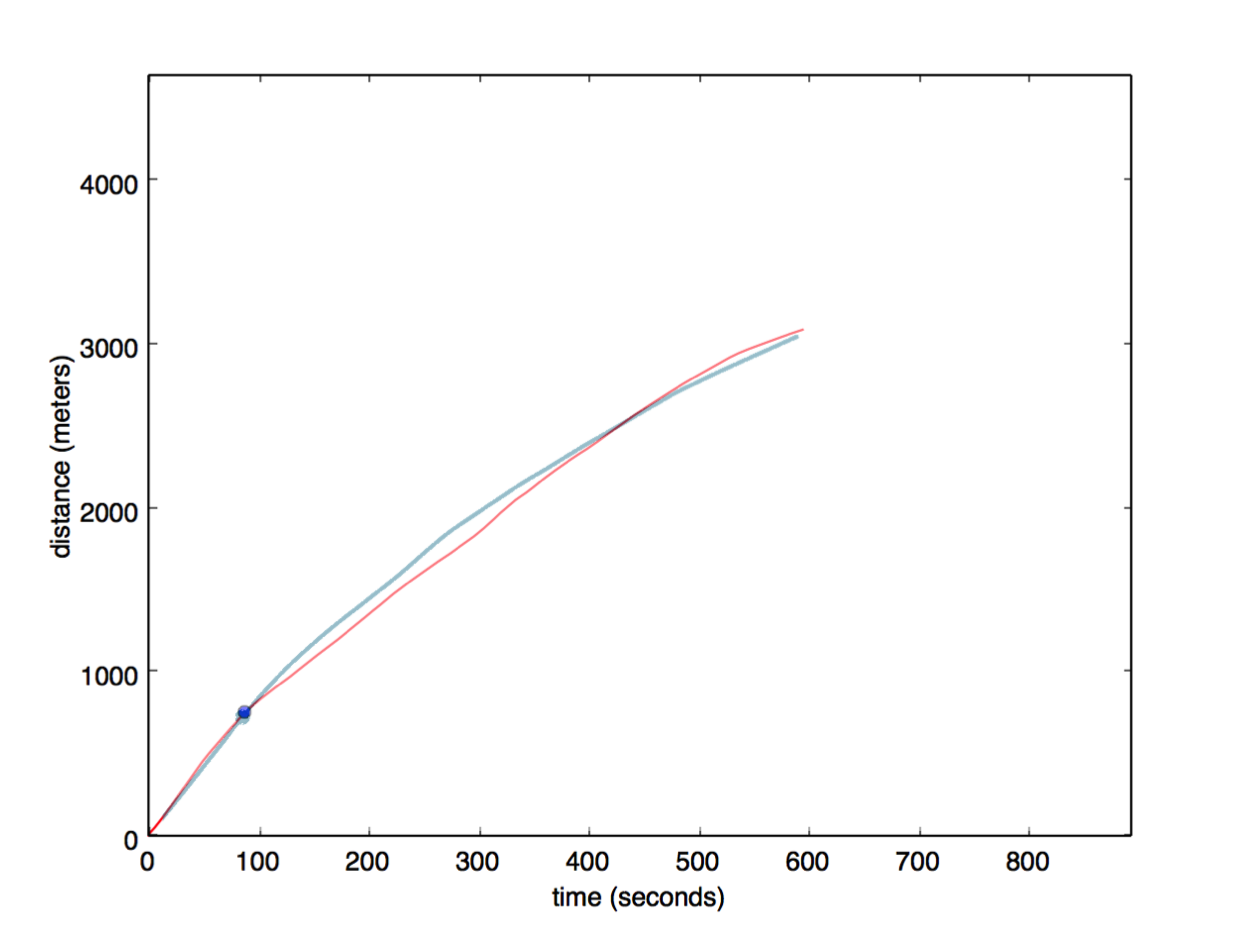
\includegraphics[width=6cm]{overlap_run.png}
\caption{A graph of pace from an actual run (shown in red) and a graph of the predicted pace (shown in blue). }
\end{center}
\end{figure}
	
	Our prediction algorithm implements a merging of our closest neighbors, iterating through each time interval for which an average of the elapsed distances is produced using geometric averaging of coordinates.  We achieve reasonable accuracy in this process by using an exponential decay weighting, by which runs further in distance from our desired prediction are given exponentially lower weighting.  By this we have our weighted output value:. We defined our gamma value such that we give a neighboring run <1\% weighting after a 5km distance from our desired output.  We believe this difference is the value at which we are considering distinctly separate types of runs.  We note that generally for every given kilometer away from our desired output, the weighting of a neighbor is essentially cut in a third.\\
	
	
	
	Using this predicted graph R(x,y,z) we provide tangent-line and secant-line predictions such that we provide a recommended pace for a runner such that given their current performance they achieve, exceed, or relax compared to their usual performance.  This step essentially merges our predictive data with the runner'��s current activity and would be the useful user-facing data provided in a retail application of our algorithms.\\
	
\begin{figure}[H]
\begin{center}
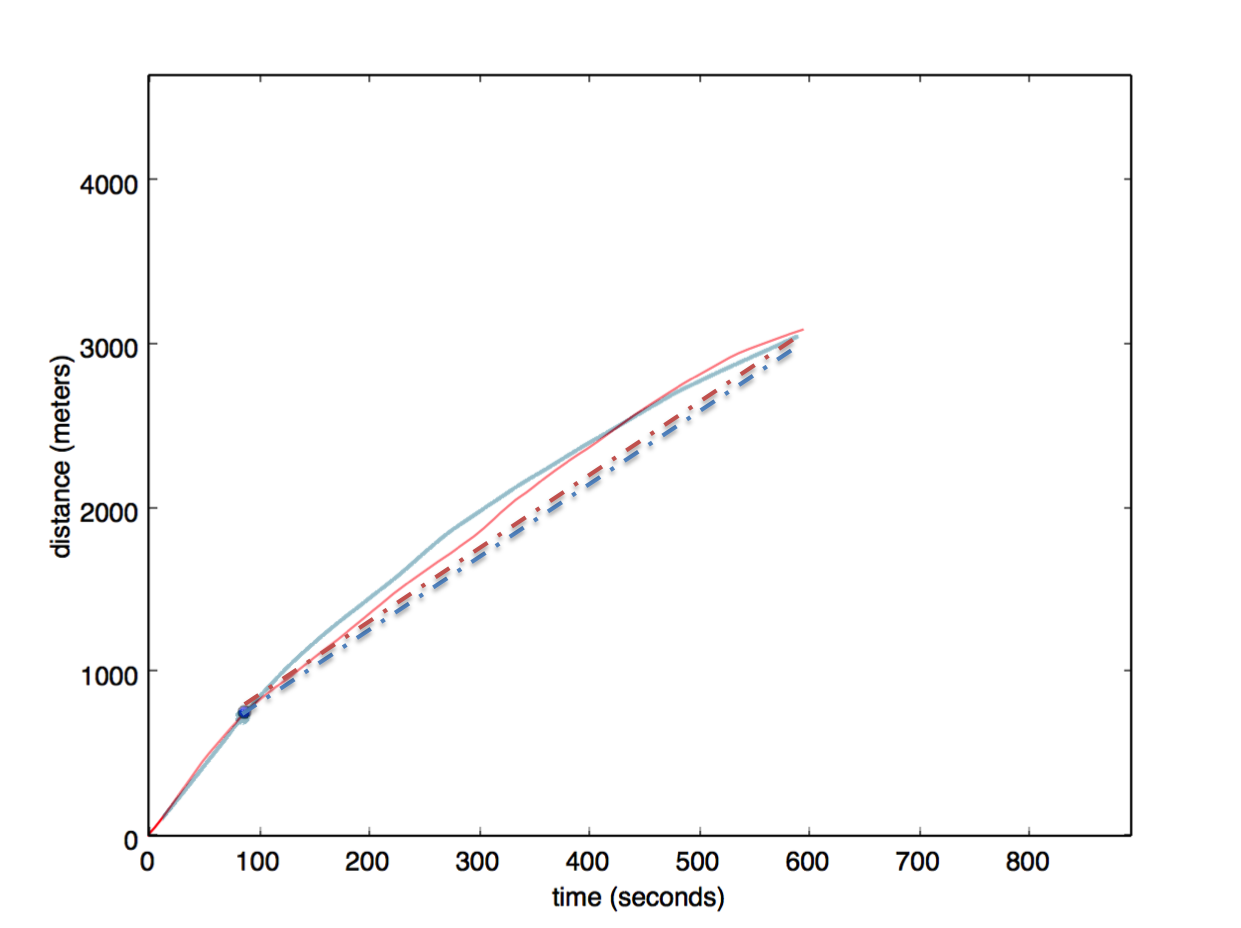
\includegraphics[width=6cm]{overlap_run_secant.png}
\caption{A graph of pace from an actual run (shown in red) and a graph of the predicted pace (shown in blue).  The secant line pace prediction is shown for the actual and predicted run in red and blue dashed lines, respectively.}
\end{center}
\end{figure}	

\subsection{Design Decisions}
	We consider again some choice design decisions made in the creation of our algorithms.  We note that for the scope of this assignment there were both many logical and arbitrary invariants we had to consider which influenced our design decisions.\\
	
	We determined that distance elapsed is the best metric of run progress after considering the alternative instantaneous speed.  It is difficult to define the term instantaneous as to produce speed a rate must be taken and therefore it is imperative to decide upon a time interval which we define as instantaneous.  Using elapsed distance allows the bypassing of this arbitrary design problem, though speed could still easily be calculated by measuring the change in elapsed distance over some defined time interval.\\
	
	We consider the tradeoff of with how many variables we represent a run and how tractable and verifiable our analysis is.  We considered a representation of n >= 4 dimensions, adding instantaneous parameters such as pace, heart rate, etc. and found that these additional parameters gave us little benefit while greatly complicating our analysis.  We found that variables time, distance elapsed, and total distance provided the simplest reasonable and most tractable effective results.\\
	
	To implement a k-nearest neighbors algorithm we had to make a best definition of nearest and determine how many neighbors to include in our analysis.  We considered other definitions of nearest but settled on comparing z-values as we assumed the invariant of good data and only comparing among the same runner such that many other variables can be ignored for the sake of our analysis.  We semi-arbitrarily came to the conclusion of using k=5 for our neighbors, determining that 5 strikes a nice balance between an accurate prediction, fast execution, and readable results.  We found that for k>=5 the quantitative benefit of additional neighbors dropped off exponentially.\\
	
	We decided to use secant and tangent lines in supplying our pace recommendation output due to their simplicity and understandability. For the purposes of our algorithms, we wanted to provide a simple metric which a runner could use as an immediate recommendation.  We considered outputting our more detailed itineraries though these are beyond the goals of our project.\\



%------------------------------------------------

\section{Results and Analysis}

\indent Given that the goal of the algorithm is predicting future pace information given current time and distance, we chose to assess the results quantitatively. The analysis involved taking a sample run (not in our database), calculating expected pace at a random point, and comparing the accuracy of our expected pace to the actual pace.\\

Here we present the full approach for measuring accuracy:

\begin{algorithm}[H]
 \KwData{Given a set of complete runs $S$}

 \For{i = 0; i < 5000; i++}{  
Choose a random run $r$ in $S$\\
Choose a random (time,distance) point in $r$ as $(t,d)$\linebreak\linebreak
Calculate the true secant line $l_t$ from $(t,d)$ to the end of the run\\
Slope($l_t$) = true average pace for the rest of the run\linebreak\linebreak
Use the SmarteRun algorithm to model a predicted run using $t$, $d$, and total distance\linebreak\linebreak
Calculate the secant line $l_p$ from $(t,d)$ to the end of the predicted run\\
Slope($l_p$) = predicted average pace for the rest of the run
 }
 Calculate error between each $l_t$ and $l_p$
 \caption{Assessing the accuracy of a run prediction}
\end{algorithm}

The purpose of this approach was to compare the accuracy of predicted pace to the actual pace for a run. Since our algorithm yields a full model of distance over time for a run, it is possible to sample multiple points along this model and compare expected pace to actual pace. We chose to use RMSE to measure accuracy because this project represents baseline accuracy; as we make changes to the algorithm in the future, we can optimize parameters with respect to minimizing RMSE.\\

Overall the results indicated a RMSE of 2.3088. As can be seen in the figure below, in general average pace was close to predicted pace (as shown by the large cluster of data points along the line $x=y$). However, clear groups of outliers exist, particularly in predicting too fast of a pace. A simple solution to reduce error would be capping the pace that we predict at $10 m/s$ (this pace represents one of the fastest human sprints, and is highly unlikely to be exceeded by recreational runners).

\begin{figure}[H]
\begin{center}
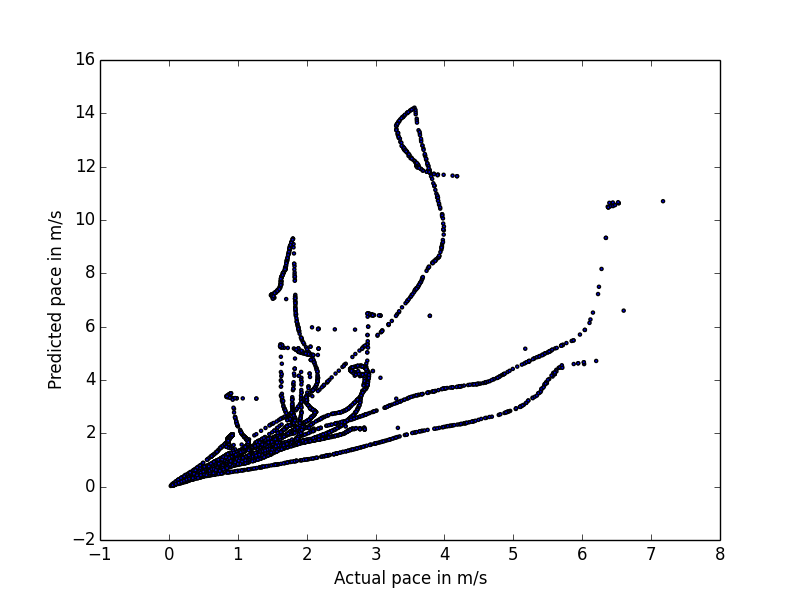
\includegraphics[width=6cm]{all.png}
\caption{A graph comparing actual pace with predicted pace. }
\end{center}
\end{figure}

However, we have two implicit truths about these predictions. The first is that predicting pace for shorter runs should be easier (more accurate) than doing so for longer runs. This is because pace can vary less over a shorter run, so we would assume less possible variance in our model. The second is that predicting pace in the second half of a run should be more accurate than doing so for the first half of the run. This is because the second half of the run is by default closer to the end, so runners? parameters have less time to change. We decided to test these two assumptions, with the specific goal of making sure that we still have reasonable accuracy over the harder of these two problems. This is also a useful benchmark, as future optimizations should not just attempt to reduce RMSE, but also attempt to increase accuracy for these harder subsets of the problem.\\
 
In the first case, we compared the accuracy of predicted pace between short runs and long runs. To do so, we repeated the algorithm presented above over a group of runs less than 3km in length as well as over a group of runs greater than 5km in length. We found a RMSE of 0.8771  for the group of short runs as compared to an RMSE of 4.0195 for the group of longer runs.

\begin{figure}[H]
\begin{center}
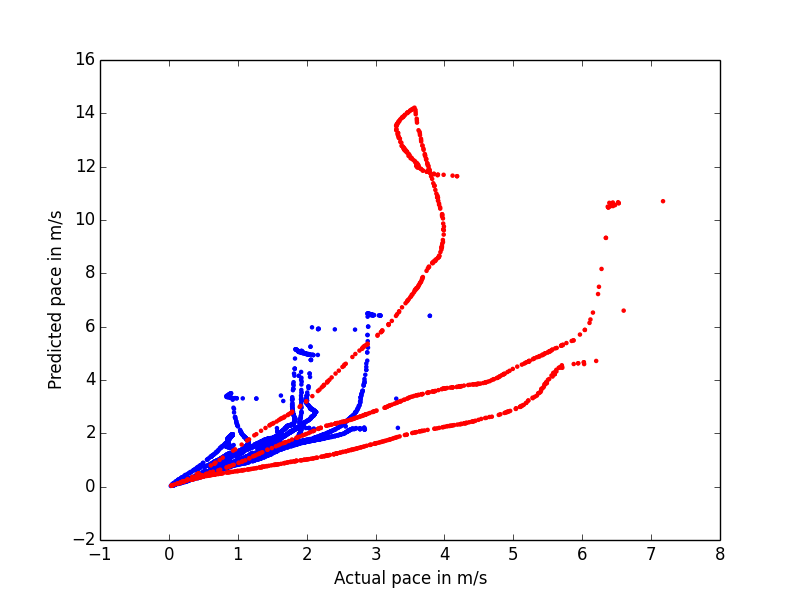
\includegraphics[width=6cm]{longshort.png}
\caption{A graph comparing actual pace with predicted pace with long runs shown in red and short runs in blue. }
\end{center}
\end{figure}
 
In the second case, we compared the accuracy of predicted pace between the predictions made in the first half and those made in the second half of runs. We used the same procedure as above, but drew random starting points from the first and second half of time values, respectively. We found a RMSE of 0.5969 for the first halves of runs as compared to an RMSE of 2.9751 for the second halves runs.

\begin{figure}[H]
\begin{center}
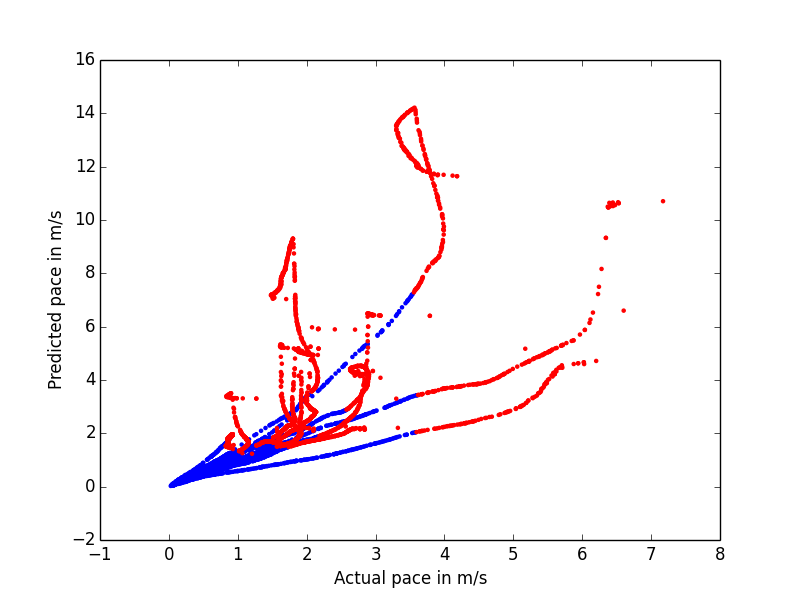
\includegraphics[width=6cm]{halves.png}
\caption{A graph comparing actual pace with predicted pace with predictions made in the first half of a run shown in blue and those in the second half of a run in red. }
\end{center}
\end{figure}



%------------------------------------------------

\section{Conclusion}

\indent This project used a K-nearest-neighbor search attempting to take past runs and combine them in reveal information about how a typical run from a user would go. This estimation is then useful in predicting a good recommendation for how the runner should progress from that moment in the run. This approach to this issue resulted in a good prediction engine for short runs and a good starting point for longer runs. The longer runs are exceedingly difficult to extrapolate to because of the many factors that can come into play over the remaining time limit as well as the limited amount of long distance run data available during this project. Having access to a good amount of RunKeeper's or MapMyRun's data would allow for much more analysis. Combining run results is a difficult task and has many points of improvement that could probably apply to non-running type exercises as well. \\

	This investigation provided useful results, but it was intended mainly as a starting point. The problem of workout recommendation is the source of entire professions (i.e. personal trainers). This project assumed all runs were "good" runs and thus should be taken into account for prediction. In reality, some runs are ruined by a bad cramp, an error in data collection, or a phone call mid-run and thus should not be used to describe typical performance. Additionally, we ran our K-nearest-neighbor algorithm on the current run and matched other runs together based on just the Z variable of total run length. This could be improved if we tried to find runs similar to the current one based on the total length as well as the performance so far. This would allow us to, at least to some degree, more properly predict the longer runs as well as fix another major development that this problem needs before anyone can call it solved: atrophy during extended periods of inactivity. This app currently assumes the user is constantly training, however, a very common use case is ignored. Namely, a runner will often take a few weeks or even months off because they are particularly busy or it's winter. This would lead to a mismatch where the runner is in much worse shape than our current algorithm understands and then tells the runner to essentially sprint the rest of the run. Matching by performance so-far in the run would allow the algorithm to implicitly match on conditioning level as well. With a large enough user base, this could become very powerful as thousands of runs can be combined from a multitude of different users, much in the same way Netflix powers their suggestion engine. Furthermore, these approaches could easily be applied to many more types of exercise such as swimming or weight lifting as well. \\
	
	With a little bit of improvement, this type of project would be very valuable to an application such as RunKeeper. Taking the expected performance and translating it into a pace that the runner should keep would be a good next step in this project. Using assumptions based on the height of the runner would be a simple way to suggest a running pace based on speed, however an entirely separate study should be done on how to use machine learning to match a specific user to the proper pace based on where they are in the run and any other factors specific to their person and their run. This could then be a powerful tool to give runners the coach they don't even know they have. 

%----------------------------------------------------------------------------------------
%	REFERENCE LIST
%----------------------------------------------------------------------------------------

\begin{thebibliography}{99} % Bibliography - this is intentionally simple in this template


\bibitem[Hammerling, Cefalu, et al., 2014]{Hammerling:2014dg}
Hammerling D, Cefalu M, Cisewski J, Dominici F, Parmigiani G, et al. (2014).
\newblock Completing the Results of the 2013 Boston Marathon. 
\newblock {\em PLoS ONE}, 9(4): e93800. doi:10.1371/journal.pone.0093800

\bibitem[Karageorghis, Costas, et al., 2013]{Karageorghis:2013dg}
Karageorghis, Costas I., Jasmin C. Hutchinson, Leighton Jones, Hannah L. Farmer, Metin S. Ayhan, Rachel C. Wilson, Joshua Rance, Christopher J. Hepworth, and Stewart G. Bailey. 
\newblock Psychological, Psychophysical, and Ergogenic Effects of Music in Swimming. 
\newblock {\em Psychology of Sport and Exercise}, 14.4 (2013): 560-68. Print.
 
\end{thebibliography}

%----------------------------------------------------------------------------------------

\end{multicols}

\end{document}
